\pagestyle{empty}


\begin{frame}{Duality  via Farkas' lemma}

  
\begin{theorem}[Second variant of Farkas' lemma]
\label{dual:thr:2farkas}
    Let $A \in \setR^{m\times n}$ and $b \in \setR^m$. The system $Ax\leq b$ has a
    solution if and only if for all $\lambda\geq0$ with $\lambda^TA =0$ one has
    $\lambda^Tb\geq0$. 
\end{theorem}

  
\end{frame}
\begin{frame}{Duality  via Farkas' lemma}


\end{frame}


\begin{frame}
  \frametitle{Algorithms and running time analysis}

  Consider the following algorithm to compute the product of two $n × n$ matrices $A,B ∈ ℚ^{n ×n}$: 
    \begin{tabbing}            
    {\bf for} \= $i=1,\dots,n$ \\ 
              \> {\bf for} \= $j=1,\dots,n$ \\
              \> \> $c_{ij} := 0$ \\
              \> \> {\bf for} \= $k=1,\dots,n$ \\
              \> \> \> $c_{ij} := c_{ij} + a_{ik} ⋅ a_{kj}$
            \end{tabbing} 
%
\end{frame}



\begin{frame}
  
\end{frame}

\begin{frame}
  \frametitle{\boldmath $O$-notation}
  
\begin{definition}

 Let $T,f: \setN \to \setR_{\geq0}$ be functions. We say 
  \begin{itemize}
  \item \emph{$T(n) = O(f(n))$}, if there exist positive  constants
    $n_o\in \setN$ and  $c\in\setR_{>0}$ 
    with $$T(n) \leq c \cdot f(n) \text{ for all }n\geq n_0.$$  
  \item \emph{$T(n) = \Omega(f(n))$}, if there exist constants   $n_o\in \setN$
    and  $c\in\setR_{>0}$ 
    with $$T(n) \geq c \cdot f(n)\text{ for all } n\geq n_0.$$
  \item \emph{$T(n) = \Theta(f(n))$}  if $$T(n)=O(f(n))\text{ and }
     T(n) = \Omega(f(n)).$$
  \end{itemize}
\end{definition}


\end{frame}


\begin{frame}{Example}

  

  \begin{example}

    \begin{itemize}
    \item $T(n)=2n^2 + 3n +1 = O(n^2)$      
    \item $T(n) = \Omega(n^2)$
    \item       $T(n) = \Theta(n^2)$.

    \item $n^2 \log n = O(n^{2 + ε} )$ for each $ε>0$ 
    \end{itemize}
\end{example}
  
\end{frame}



\begin{frame}{Efficient algorithm, first definition}

  \begin{definition}[Polynomial-time algorithm] 
    An algorithm runs in
\emph{polynomial time}, if there exists a constant $k$ such that the
algorithm runs in time
\begin{displaymath}
  O(n^k)
\end{displaymath}
where $n$ is the length of the input  (total number of bits). 

  \end{definition}
  
\end{frame}


\begin{frame}{Why  definition is problematic} 
  
\end{frame}


\begin{frame}{}


  \begin{columns}
    \begin{column}{.5\textwidth}
      
    \end{column}
    \begin{column}{.5\textwidth}
      
    \end{column}       
  \end{columns}
\end{frame}



\begin{frame}{Size}

\begin{definition}
  \label{def:2}
  The \emph{size} of an integer $x$
  is $\size(x) = \lceil\log( |x| +1)\rceil$
  and for $x \in \setQ$,
  $\size(x) = \size(p)+\size(q)$,
  where $x = p/q$ with $p,q \in \setZ$, $q\geq1$ and $\gcd(p,q)=1$.   
\end{definition}


  \begin{columns}
    \begin{column}{.5\textwidth}
      
    \end{column}
    \begin{column}{.5\textwidth}
      
    \end{column}       
  \end{columns}
\end{frame}



\begin{frame}{Polynomial time algorithm}

  \begin{definition}
  \label{def:1}
  An algorithm is \emph{polynomial time}, if there exists a
  constant $k$
  such that the algorithm performs $O(n^k)$
  operations on rational numbers whose size is bounded by
  $O(n^k)$.
  Here $n$
  is the number of bits that encode the input of the algorithm. We say that the algorithm runs in time $O(n^k)$. 
\end{definition}
\end{frame}

\begin{frame}{Example: Euclidean algorithm}


  \begin{tabbing}
      Input: Integers $a ≥ b ≥0$ not both equal to zero \\
      Output: The greatest common divisor $\gcd(a,b)$\\[2ex]
      {\bf if}  $(b=0)$ {\bf return} $a$ \\
      {\bf else} \= \\
      \> Compute $q,r ∈ ℕ$ with \=  $b > r ≥ 0$ and $a = q⋅b +r$ \\
      \> \> (division with remainder)\\
      \> {\bf return} $\gcd(b,r)$ 
    \end{tabbing}
   \begin{columns}
    \begin{column}{.5\textwidth}
      
    \end{column}
    \begin{column}{.5\textwidth}
      
    \end{column}       
  \end{columns}
\end{frame}



\begin{frame}{Analysis}


  \begin{columns}
    \begin{column}{.5\textwidth}
      
    \end{column}
    \begin{column}{.5\textwidth}
      
    \end{column}       
  \end{columns}
\end{frame}



\begin{frame}{Determinant}

\begin{tabbing}
  Input: $A ∈ ℚ^{n  ×n}$ \\
  Output: $\det(A)$ \\
  
  {\bf if} \= $(n=1)$ \\
           \> {\bf return} $a_{11}$ \\
  {\bf else} \\
           \> $d:=0$  \\
           \> {\bf for } \= $j=1,\dots,n$ \\
           \>            \> $d:= (-1)^{1+j}⋅ \det(A_{1j}) +d$\\
           \> {\bf return} $d$   
         \end{tabbing}

         
  \begin{columns}
    \begin{column}{.5\textwidth}
      
    \end{column}
    \begin{column}{.5\textwidth}
      
    \end{column}       
  \end{columns}
\end{frame}




\begin{frame}{Analysis}


\begin{figure}
  \centering
  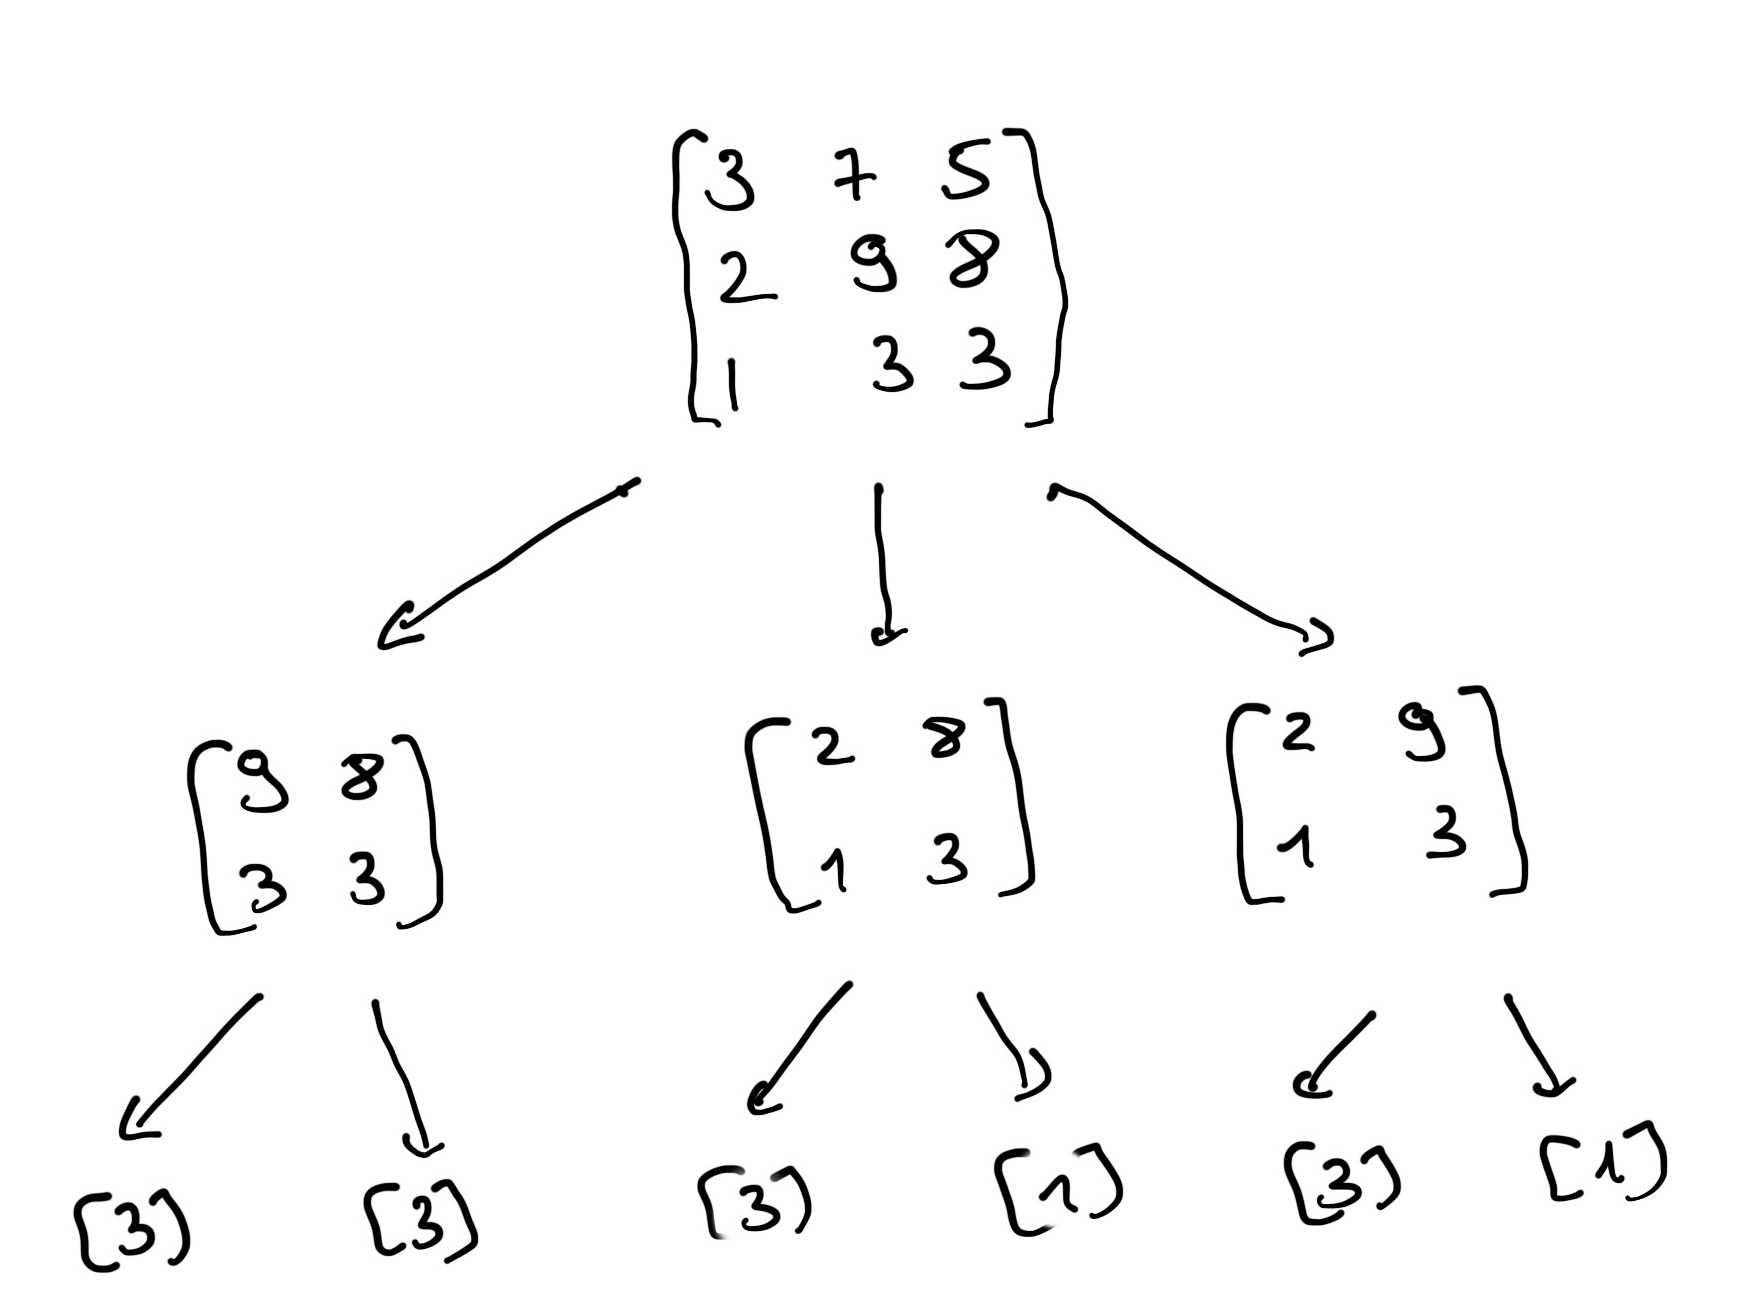
\includegraphics[height=5cm]{../figures/DeterminantAlgoSlow.jpg}
  \caption{An example of the recursion tree of the algorithm from Example~\ref{exe:det}. The tree corresponds to the run of the algorithm on input $\protect\smat{         3 & 7 & 5 \\ 2&9&8 \\ 1 & 3 & 3  }.$
} 
\end{figure}


  \begin{columns}
    \begin{column}{.5\textwidth}
      
    \end{column}
    \begin{column}{.5\textwidth}
      
    \end{column}       
  \end{columns}
\end{frame}



\begin{frame}{Gaussian elimination}

  \begin{tabbing}
    Input: $A ∈ ℚ^{m ×n}$  \\
    Output: \= $A'$ in row echelon form such that there exists an invertible \\ 
            \> $Q ∈ ℚ^{m × m}$ such that $Q⋅A = A'$ . \\[1ex]
            \pushtabs 
$A' := A$ \\
$i := 1$\\
{\bf while} \=  ($i≤m$)  \\
\> find \emph{minimal} $1 ≤ j ≤n$ such that there exists $k≥i$ such that $a'_{kj} ≠ 0$ \\
\> If no such element exists, then {\bf stop} \\
            \> swap rows $i$ and $k$ in $A'$ \\
            \>  {\bf for} \= $k = i+1,\dots, m$ \\
            \>            \> subtract $(a'_{kj}/a'_{ij})$ times row $i$ from row $k$ in $A'$  \\
\> $i:=i+1$ 
\poptabs        
  \end{tabbing}
  \begin{columns}
    \begin{column}{.5\textwidth}
      
    \end{column}
    \begin{column}{.5\textwidth}
      
    \end{column}       
  \end{columns}
\end{frame}



\begin{frame}{Analysis}

\begin{theorem}
  \label{thr:9}
The   Gaussian algorithm runs in polynomial time on input $A ∈ ℤ^{m ×n}$.  More precisely, the rational numbers produced in the algorithm can be maintained to be  ratios of sub-determinants of $A'$ and are thus of polynomial binary encoding length. 
\end{theorem}

  \begin{columns}
    \begin{column}{.5\textwidth}
      
    \end{column}
    \begin{column}{.5\textwidth}
      
    \end{column}       
  \end{columns}
\end{frame}






\begin{frame}{}


  \begin{columns}
    \begin{column}{.5\textwidth}
      
    \end{column}
    \begin{column}{.5\textwidth}
      
    \end{column}       
  \end{columns}
\end{frame}



\begin{frame}{Matrix multiplication}

  
If we split the matrices $A$ and $B$ into 4 $n/2 × n/2$ matrices 
\begin{equation}
  \label{eq:str:3}
  A =
  \begin{pmatrix}
    A_{11} & A_{12} \\ 
    A_{21} & A_{22} 
  \end{pmatrix} \, \text{ and }  B =
  \begin{pmatrix}
    B_{11} & B_{12} \\ 
    B_{21} & B_{22} 
  \end{pmatrix}
\end{equation}
Then 
\begin{displaymath}
  \begin{pmatrix}
    C_{11} & C_{12} \\
    C_{21} & C_{22}
  \end{pmatrix}
   =
  \begin{pmatrix}
    A_{11}\cdot B_{11} + A_{12}\cdot B_{21} & \, &  A_{11}\cdot B_{12} + A_{12}\cdot B_{22}  \\
        A_{21}\cdot B_{11} + A_{22}\cdot B_{21} &\, &     A_{21}\cdot B_{12} + A_{22}\cdot B_{22} 
  \end{pmatrix}.
\end{displaymath}


  \begin{columns}
    \begin{column}{.5\textwidth}
      
    \end{column}
    \begin{column}{.5\textwidth}
      
    \end{column}       
  \end{columns}
\end{frame}



\begin{frame}{Strassen's algorithm}




  \begin{columns}
    \begin{column}{.5\textwidth}
      \begin{eqnarray*}
  M_1 & = & (A_{11} + A_{22}) \cdot (B_{11}+ B_{22}) \\
  M_2 & = & (A_{21} + A_{22}) \cdot B_{11} \\
  M_3 & = & A_{11} \cdot (B_{12} - B_{22}) \\
  M_4 & = & A_{22} \cdot (B_{21} - B_{11}) \\
  M_5 & = & (A_{11} + A_{12})\cdot B_{22} \\
  M_6 & = & (A_{21}-A_{11}) \cdot (B_{11}+B_{12}) \\
  M_7 & = & (A_{12}-A_{22}) \cdot  (B_{21} + B_{22})\\. 
\end{eqnarray*}

    \end{column}
    \begin{column}{.5\textwidth}
      \begin{eqnarray*}
C_{11} & = & M_1 + M_4 - M_5 + M_7\\
C_{12} & = & M_3 + M_5 \\
C_{21} & = & M_2 + M_4\\
C_{22} & = & M_1 - M_2 + M_3 + M_6.  
\end{eqnarray*}
    \end{column}       
  \end{columns}
\end{frame}







\begin{frame}{}


  \begin{columns}
    \begin{column}{.5\textwidth}
      
    \end{column}
    \begin{column}{.5\textwidth}
      
    \end{column}       
  \end{columns}
\end{frame}



\begin{frame}{Strassen's algorithm}
 \begin{tabbing}
    Input: Two $n ×n$ matrices $A$ and $B$ \\
    Output: $C = \mathrm{FMM}(A,B)$, the product $ A\cdot B$ \\[1ex]

    {\bf if}  $n=1$ return $a_{11} ⋅b_{11}$ \\
    {\bf else} \=  \\
               \>  $M_1 = \mathrm{FMM} (A_{11} + A_{22} , B_{11}+ B_{22}) $ \\
               \> $M_2 = \mathrm{FMM}(A_{21} + A_{22},  B_{11})$ \\
               \> $M_3  = \mathrm{FMM} A_{11} , B_{12} - B_{22}) $\\
               \> $M_4  = \mathrm{FMM}( A_{22} , (B_{21} - B_{22})$ \\
               \> $M_5  = \mathrm{FMM}(A_{11} + A_{12}, B_{22})$ \\
               \> $M_6  = \mathrm{FMM} (A_{21}-A_{11}, B_{11}+B_{12}) $\\
               \> $M_7  = \mathrm{FMM} (A_{12}-A_{22}, B_{21} + B_{22})$\\ 
               \> Compute the matrices $C_{11}, C_{12}, C_{21}, C_{22}$ from $M_1,\dots,M_7$ \\
               \> {\bf return} $C$
  \end{tabbing}

  \begin{columns}
    \begin{column}{.5\textwidth}
      
    \end{column}
    \begin{column}{.5\textwidth}
      
    \end{column}       
  \end{columns}
\end{frame}



\begin{frame}{Analysis}

  \begin{figure}
    \centering
     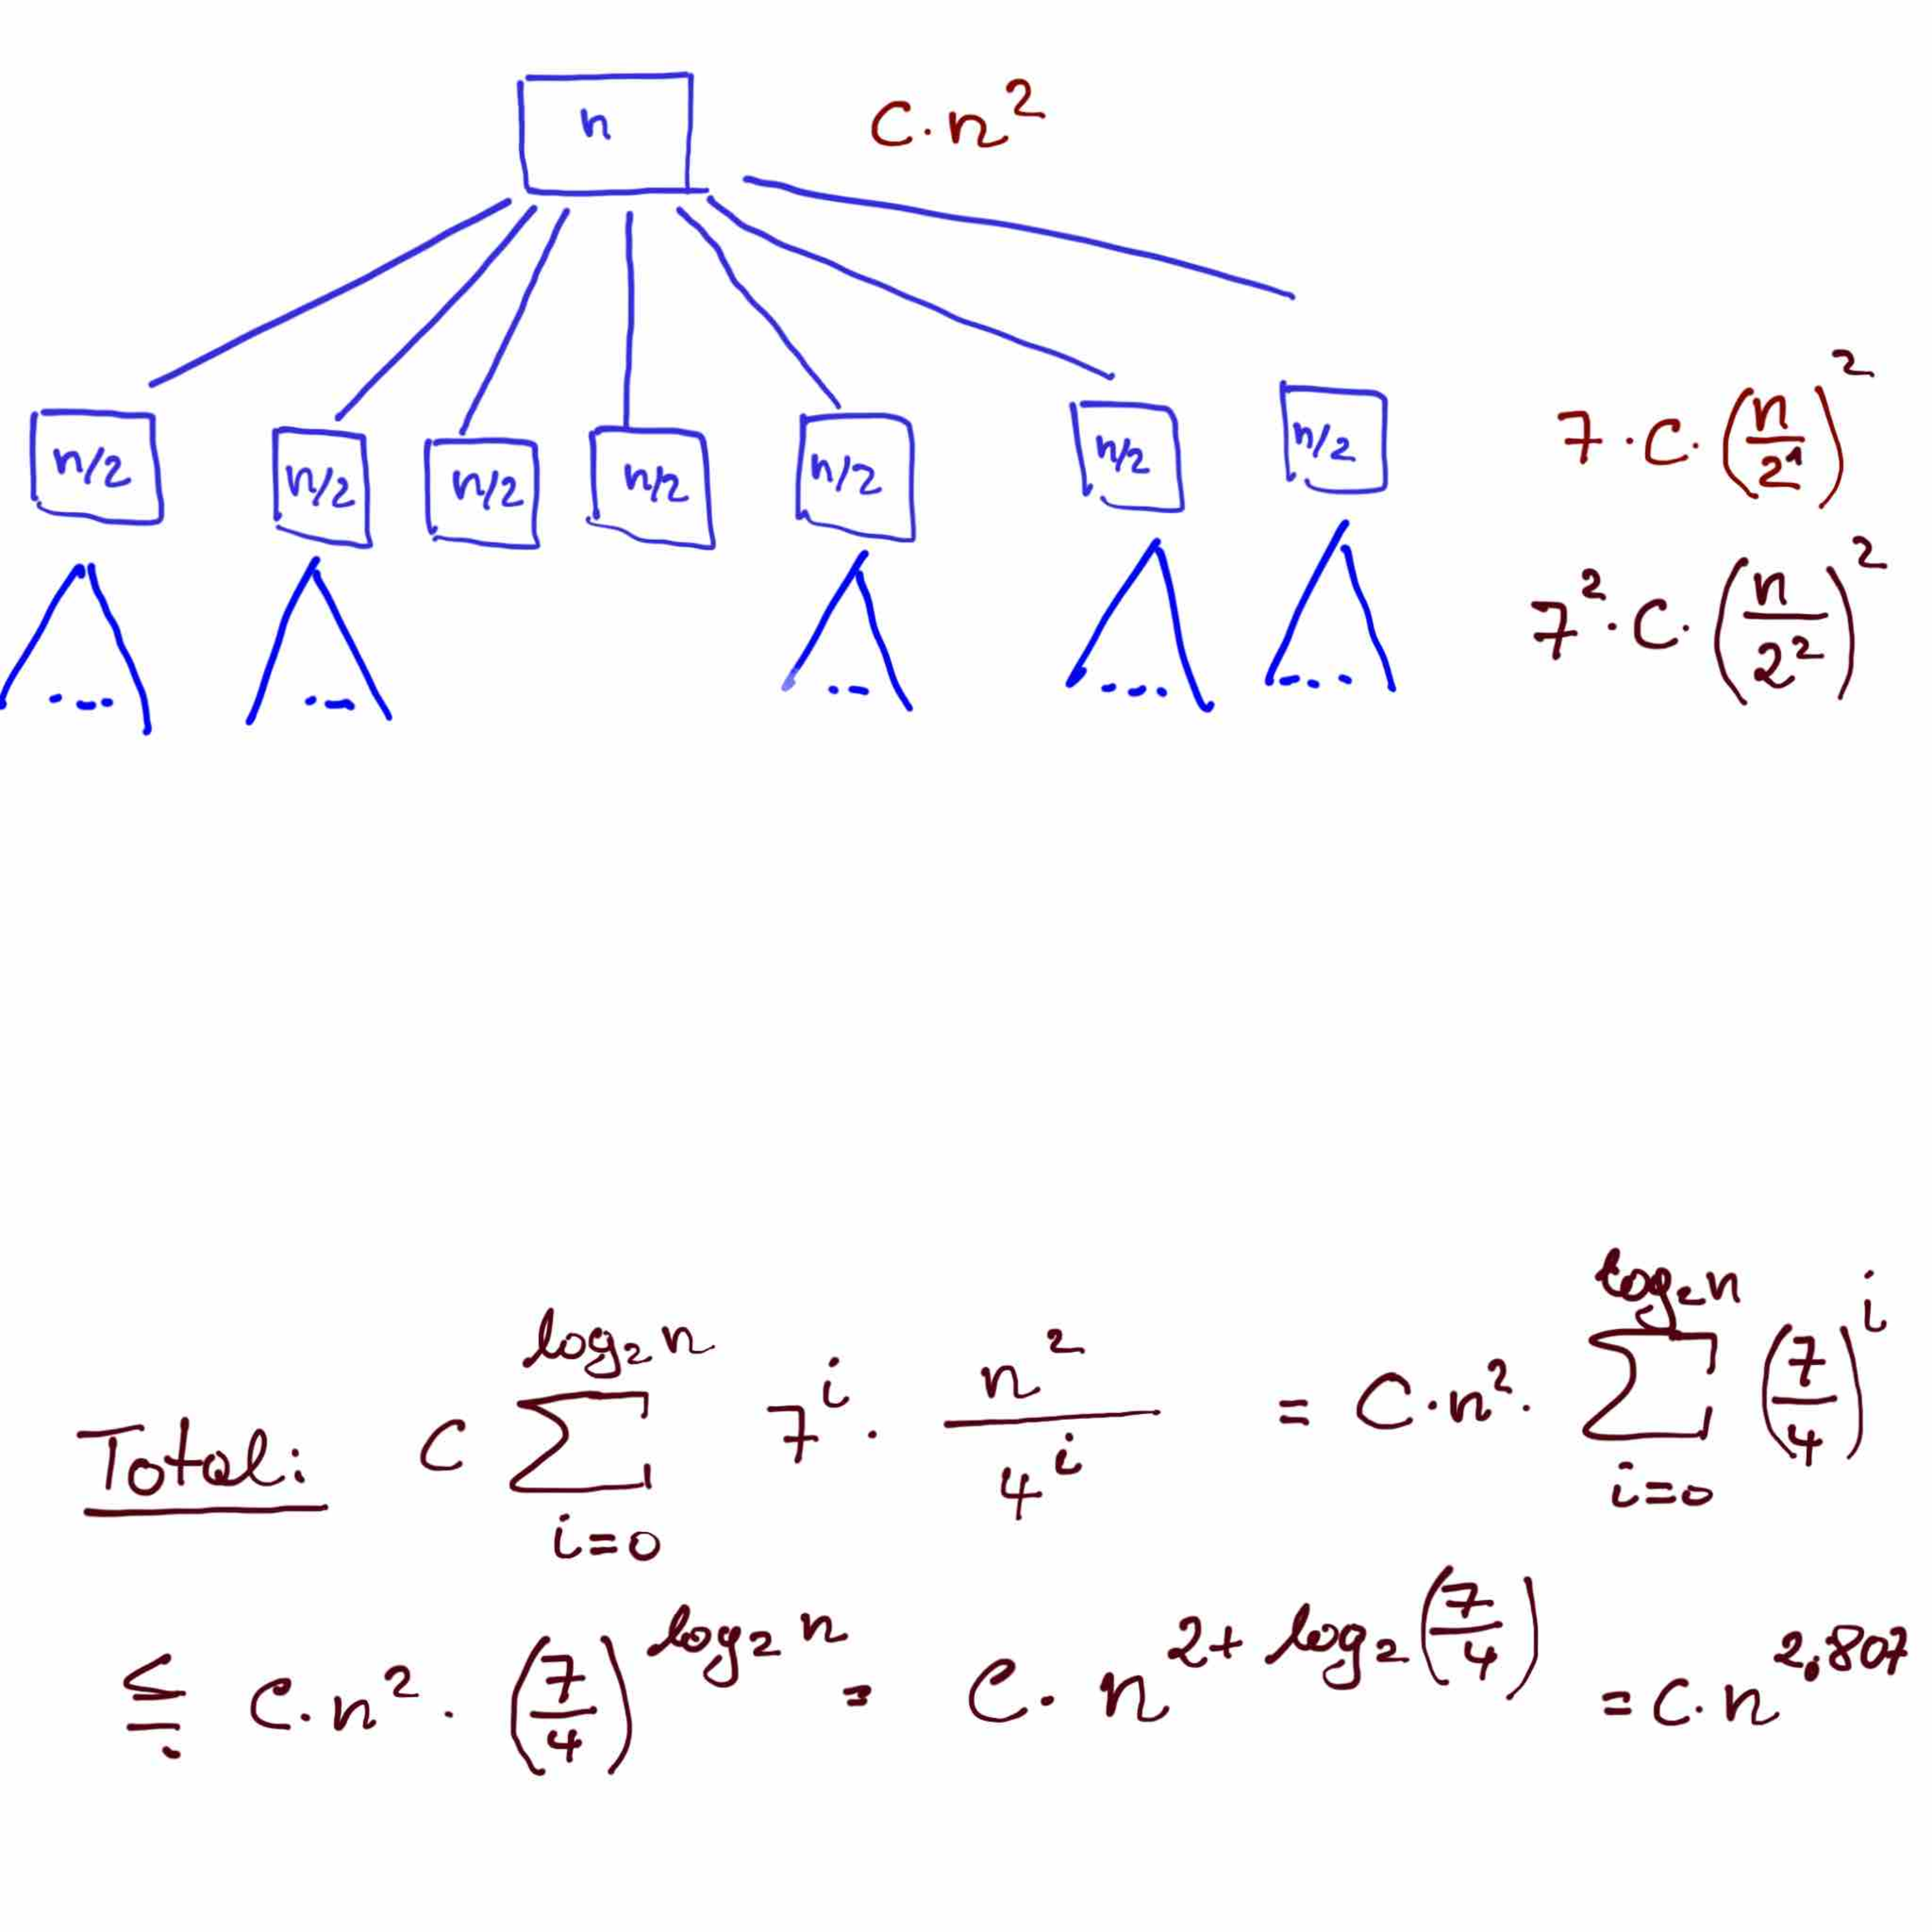
\includegraphics[height=8cm]{../figures/Strassen2.pdf} 
    \caption{The analysis of the Strassen algorithm. }
    \label{fig:str:1}
  \end{figure}



  \begin{columns}
    \begin{column}{.5\textwidth}
      
    \end{column}
    \begin{column}{.5\textwidth}
      
    \end{column}       
  \end{columns}
\end{frame}






\begin{frame}{}


  \begin{columns}
    \begin{column}{.5\textwidth}
      
    \end{column}
    \begin{column}{.5\textwidth}
      
    \end{column}       
  \end{columns}
\end{frame}



\begin{frame}{Running time}


  \begin{theorem}[Strassen]
    \label{thr:10}
    Two $n × n$ matrices can be multiplied in time (number of arithmetic operations) $O(n^{2+ \log_2(7/4)})$. 
  \end{theorem}

  

  \begin{columns}
    \begin{column}{.5\textwidth}
      
    \end{column}
    \begin{column}{.5\textwidth}
      
    \end{column}       
  \end{columns}
\end{frame}



\begin{frame}{}


  \begin{columns}
    \begin{column}{.5\textwidth}
      
    \end{column}
    \begin{column}{.5\textwidth}
      
    \end{column}       
  \end{columns}
\end{frame}




%%% Local Variables:
%%% mode: LaTeX
%%% TeX-master: "Slides"
%%% End:


